\documentclass[11pt]{article}
\usepackage[a4paper,margin=2.5cm]{geometry}
\usepackage{amsmath,amssymb}
\usepackage{booktabs}
\usepackage{graphicx}

\newcommand{\R}{\mathcal R_0}

\title{Numerical Simulations of the SVIR Model\\
with Vaccination: Bistability and the Basin Separatrix\\(prepared prompting Claude AI)}
\date{}

\begin{document}
\maketitle

\begin{abstract}
We integrate numerically an SVIR model with waning vaccine protection and waning immunity, with a vaccination rate $\phi$ chosen so that the controlled reproduction number $r$ lies in the bistability window $(r_2,1)$ predicted by the quadratic equilibrium analysis. For $\phi=0.0085$ ($r\approx0.9813$) the disease-free equilibrium and an endemic equilibrium ($I\approx0.0237$) are both stable. Initial conditions with no vaccinated individuals converge to the endemic state, initial conditions near the vaccinated disease-free state may converge to either, and we compute the curve in the $(V_0,I_0)$ plane that separates the two basins of attraction.
\end{abstract}

%=====================================================================
\section{Model and parameters}
%=====================================================================

\subsection{Equations}

The population is normalized to $N=1$ and divided into susceptible $S$, vaccinated $V$, infected $I$ and recovered $R$ individuals:
\begin{align}
\dot S &= \mu N-\beta SI-\mu S-\phi S+\theta V+\psi R,\nonumber\\
\dot V &= \phi S-(\mu+\theta)V-\sigma\beta VI,\label{eq:sys}\\
\dot I &= \beta SI+\sigma\beta VI-\gamma I-\mu I,\nonumber\\
\dot R &= \gamma I-(\mu+\psi)R.\nonumber
\end{align}
Adding the four equations gives $\dot S+\dot V+\dot I+\dot R=\mu\big(N-S-V-I-R\big)$, so $S+V+I+R=1$ is invariant. Here $\phi$ is the vaccination rate, $\theta$ the rate of loss of vaccine protection, $\sigma=1-\epsilon$ the relative susceptibility of vaccinated individuals ($\epsilon$ is the vaccine efficacy), and $\psi$ the rate of loss of natural immunity.

\subsection{Parameter values}

\begin{center}
\begin{tabular}{ll}
\toprule
Parameter & Value\\
\midrule
$\mu$ & $360\times10^{-7}$\\
$\gamma$ & $1/7$\\
$\psi$ & $1/90$\\
$\theta$ & $1/1095$\\
$\epsilon$, $\sigma$ & $0.8$, $0.2$\\
$\R$ & $3.5$\\
$\beta$ & $\R(\mu+\gamma)\approx0.500126$\\
$\phi$ & $0.0085$ (main runs); $0.00854$ (preliminary runs)\\
\bottomrule
\end{tabular}
\end{center}

\subsection{Disease-free equilibrium and the controlled reproduction number}

The disease-free equilibrium (DFE) is
\begin{equation}
S^*=\frac{\mu+\theta}{\mu+\theta+\phi},\qquad V^*=\frac{\phi}{\mu+\theta+\phi},\qquad I^*=R^*=0 .
\label{eq:dfe}
\end{equation}
Linearizing the $I$-equation at \eqref{eq:dfe} gives $\dot I=(\gamma+\mu)(r-1)I$ with
\begin{equation}
r=\frac{\beta(S^*+\sigma V^*)}{\gamma+\mu}=\R\,\frac{(\mu+\theta)+\sigma\phi}{\mu+\theta+\phi},
\qquad\text{equivalently}\qquad
\phi=(\mu+\theta)\frac{\R-r}{r-\R\sigma}.
\label{eq:r}
\end{equation}
The second relation is the function $\phi(r)$ used in the equilibrium analysis. The DFE is locally stable for $r<1$. The endemic equilibria satisfy the quadratic $AI^2+B(r)I+C(r)=0$ studied in the companion analysis, where $\R\sigma=0.7<1<\R$.

For $\beta=0.5$ the discriminant numerator $N$ has roots $r_1\approx0.728$ and $r_2\approx0.944$, and the reverse bifurcation is folded at $r_2$: for $r\in(r_2,1)$ the DFE ($r<1$) coexists with two endemic equilibria $I_1(r)>I_2(r)>0$, the upper one stable. Both choices of $\phi$ used below correspond to $r$ in this window:
\begin{itemize}
\item $\phi=0.0085$ gives $r\approx0.9813$ by \eqref{eq:r};
\item the preliminary runs used $r=0.98$, i.e.\ $\phi=0.008543$ (this value was used before the value $0.0085$ was specified).
\end{itemize}
At $\phi=0.0085$, $S^*\approx0.1005$, $V^*\approx0.8995$, and the endemic equilibrium has $I\approx0.02367$.

\subsection{Numerical method}

System \eqref{eq:sys} was integrated on $t\in[0,3000]$ with the LSODA method (scipy \texttt{solve\_ivp}, tolerances $10^{-10}$ relative and $10^{-13}$ absolute). In all runs the conserved total $S+V+I+R$ stayed equal to $1$ to machine accuracy. Curves are colored: $S$ green, $V$ orange, $I$ red, $R$ blue.

%=====================================================================
\section{Runs with no vaccinated individuals at $t=0$}
%=====================================================================

The two initial conditions are
\[
\text{(i) } S_0=0.99,\ I_0=0.01,\qquad \text{(ii) } S_0=0.9,\ I_0=0.1,\qquad V_0=R_0=0 .
\]

\subsection{Preliminary runs ($r=0.98$, $\phi\approx0.00854$)}

As a first choice, $\phi$ was computed from $r=0.98$, which lies inside the bistability window $(r_2,1)$.

\begin{figure}[ht]
\centering
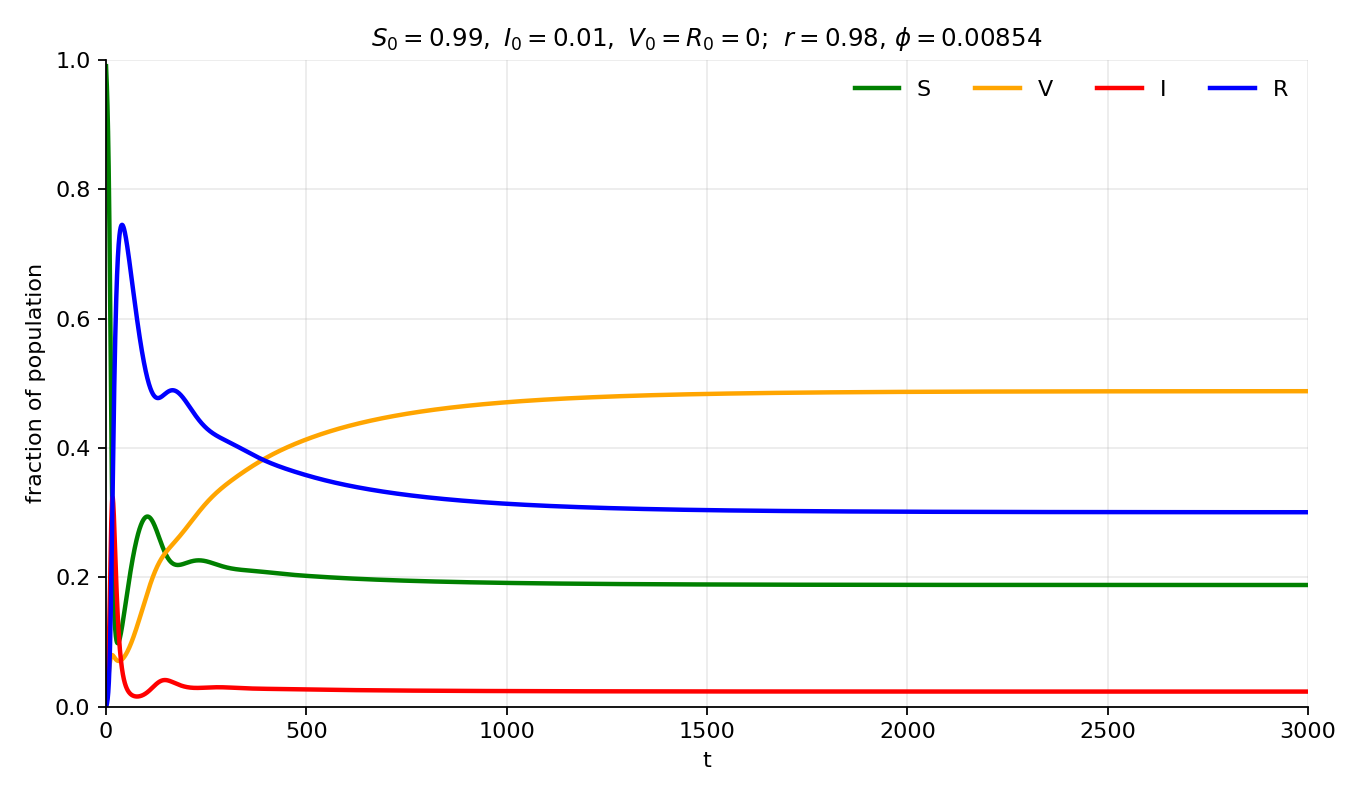
\includegraphics[width=0.48\textwidth]{sim_ic1.png}\hfill
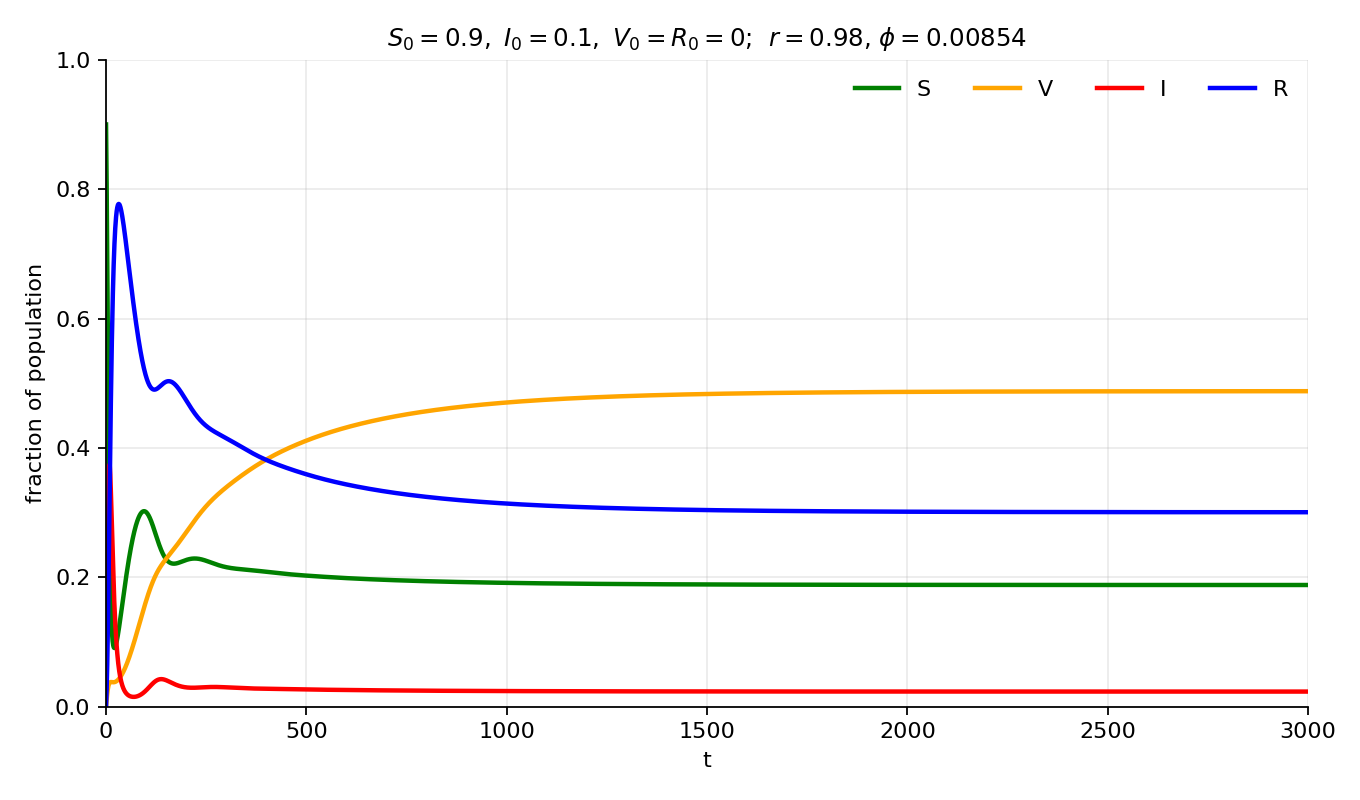
\includegraphics[width=0.48\textwidth]{sim_ic2.png}
\caption{Preliminary runs, $r=0.98$ ($\phi\approx0.00854$). Left: initial condition (i). Right: initial condition (ii).}
\label{fig:prelim}
\end{figure}

\emph{Comments.} Both runs converge to the same endemic state, $S\approx0.188$, $V\approx0.488$, $I\approx0.02346$, $R\approx0.301$. This value of $I$ agrees with the larger root $I_1(0.98)=0.023456$ of the equilibrium quadratic, which checks the consistency of the simulation with the algebraic analysis. The infection peak is $I\approx0.324$ at $t=16$ in run (i) and $I\approx0.374$ at $t=8.5$ in run (ii), followed by damped oscillations. Even much smaller initial infections ($I_0$ down to $10^{-6}$, still with $V_0=0$) end at the endemic state.

\subsection{Main runs ($\phi=0.0085$, $r\approx0.9813$)}

\begin{figure}[ht]
\centering
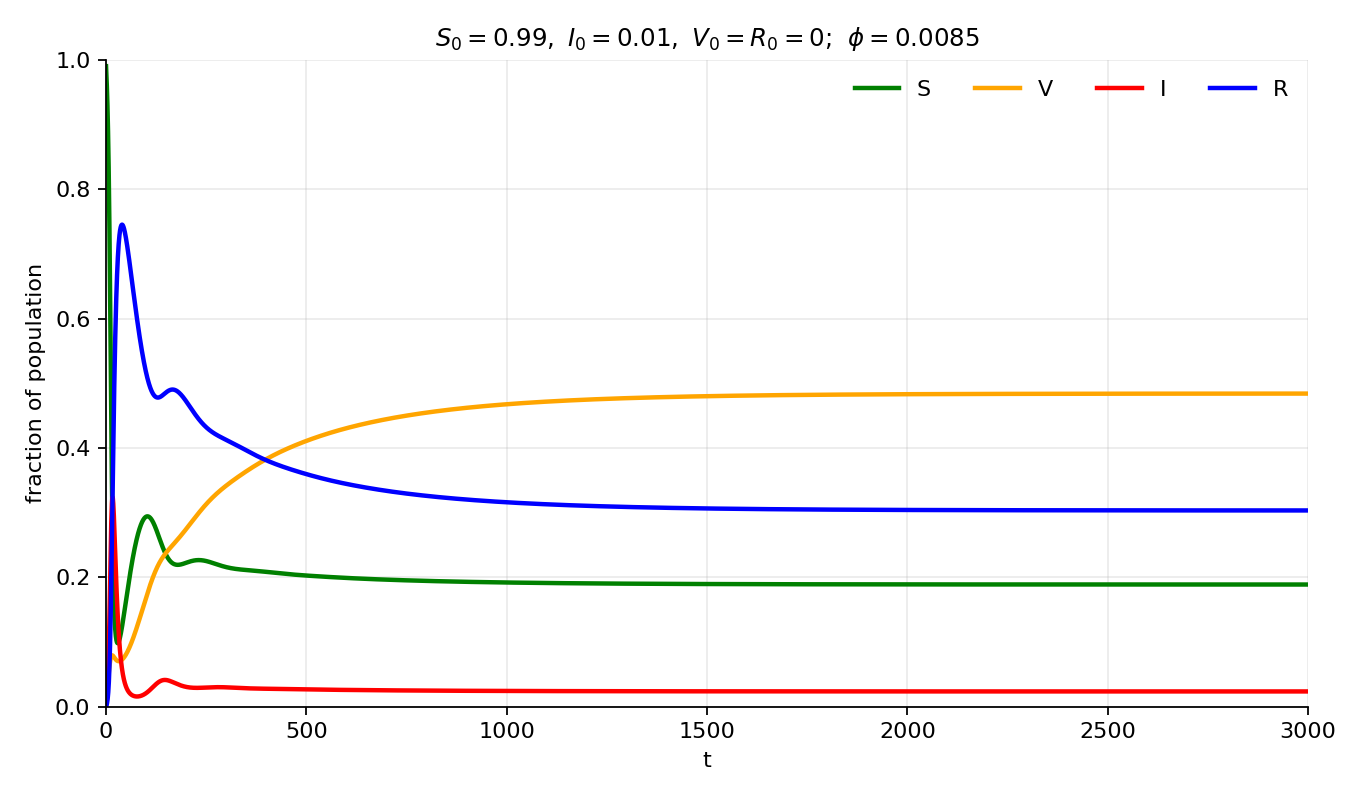
\includegraphics[width=0.85\textwidth]{sim_phi0085_ic1.png}
\caption{$\phi=0.0085$, initial condition (i): $S_0=0.99$, $I_0=0.01$, $V_0=R_0=0$.}
\label{fig:ic1}
\end{figure}

\begin{figure}[ht]
\centering
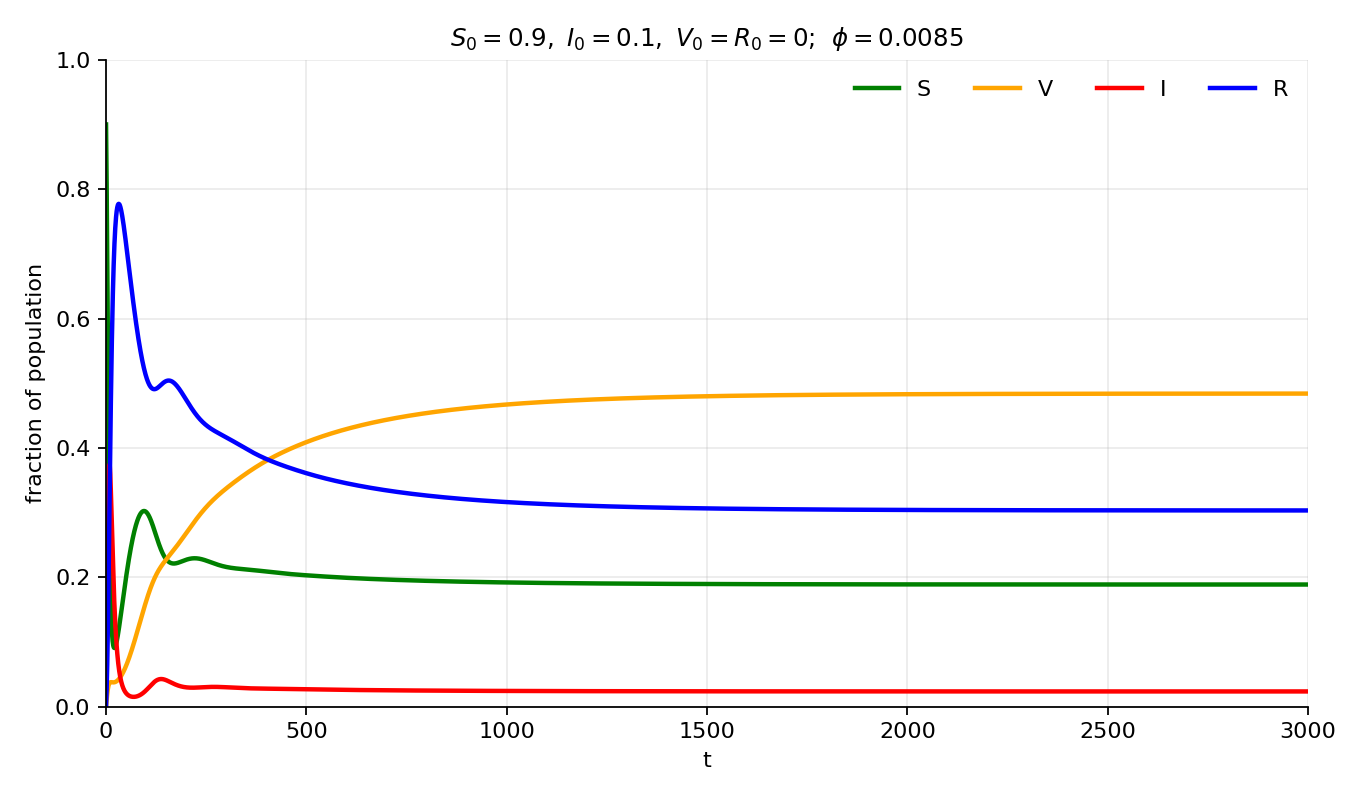
\includegraphics[width=0.85\textwidth]{sim_phi0085_ic2.png}
\caption{$\phi=0.0085$, initial condition (ii): $S_0=0.9$, $I_0=0.1$, $V_0=R_0=0$.}
\label{fig:ic2}
\end{figure}

\emph{Comments.} Again both runs end at the same endemic equilibrium: at $t=3000$, $S\approx0.1889$, $V\approx0.4840$, $I\approx0.02367$, $R\approx0.3034$, to be compared with the equilibrium value $I=0.023670$ from the quadratic. The infection peaks at $I\approx0.324$ ($t=16$) in run (i) and $I\approx0.374$ ($t=8.5$) in run (ii). Starting from $V_0=0$ the system is far from the vaccinated DFE, so it always reaches the endemic state in these experiments.

%=====================================================================
\section{The disease-free alternative}
%=====================================================================

To see the other attractor we start at the vaccinated DFE \eqref{eq:dfe} with a small infection: $S_0=S^*(1-I_0)\approx0.1004$, $V_0=V^*(1-I_0)\approx0.8986$, $I_0=0.001$, $R_0=0$ (so that $S_0+V_0+I_0=1$).

\begin{figure}[ht]
\centering
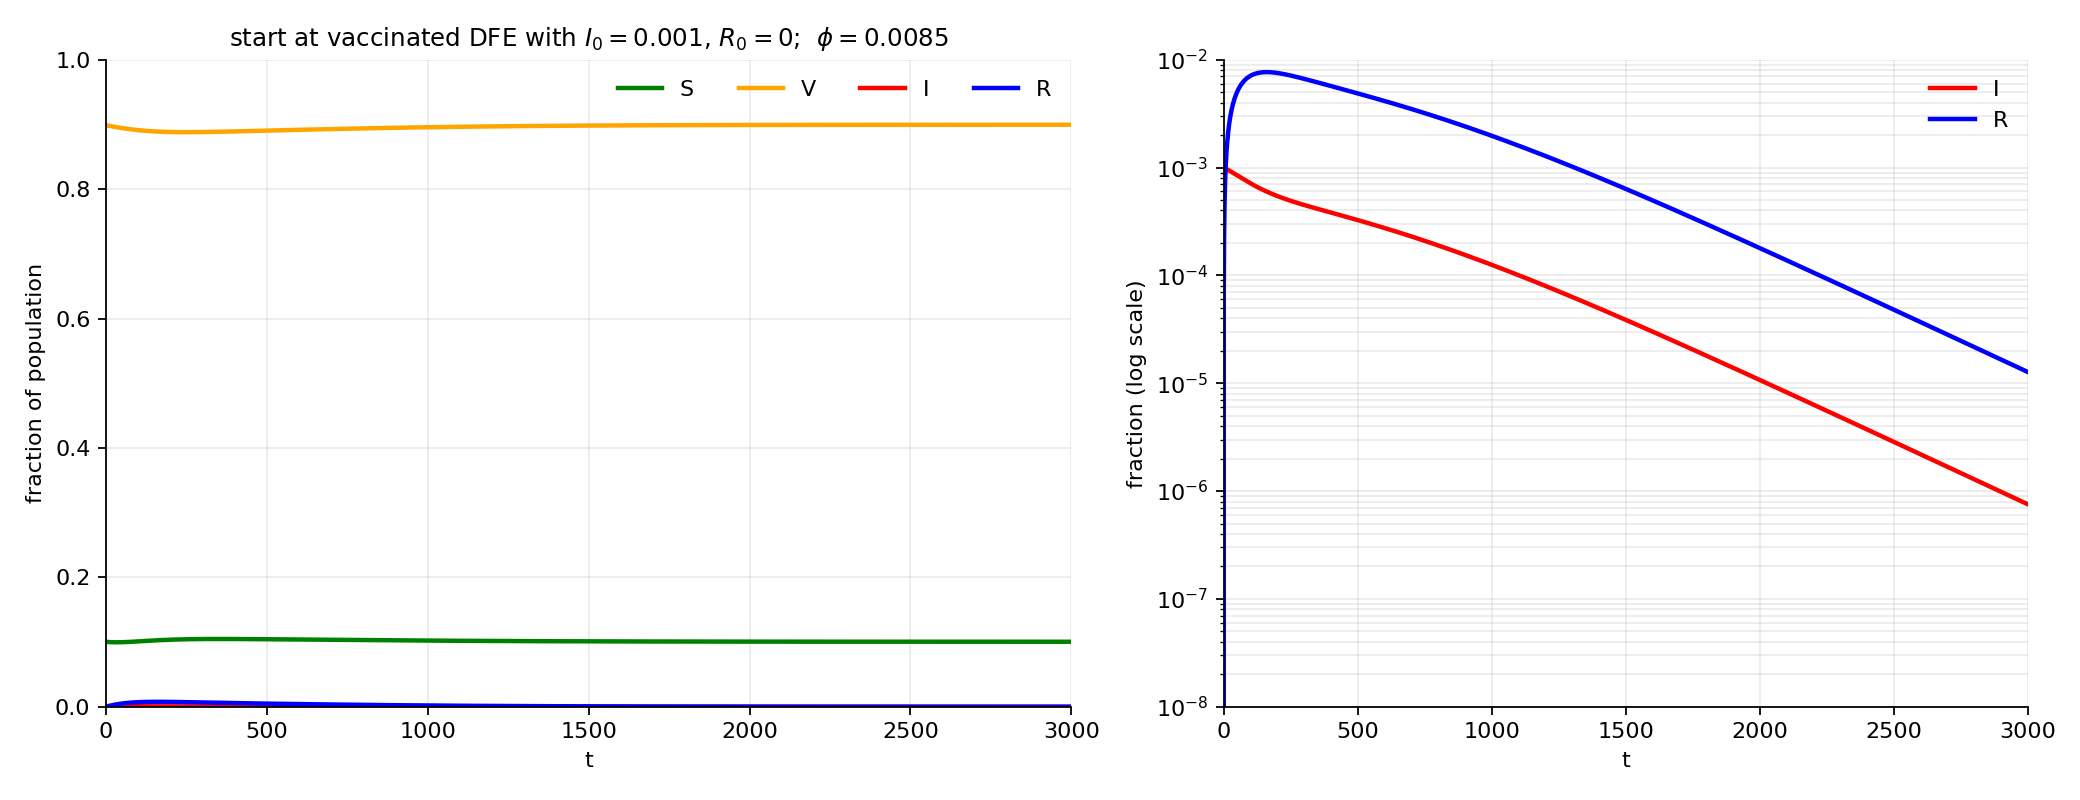
\includegraphics[width=\textwidth]{sim_phi0085_dfe.png}
\caption{Disease-free alternative, $\phi=0.0085$. Left: all compartments (the curves $I$ and $R$ are too small to see at this scale). Right: $I$ and $R$ on a logarithmic scale.}
\label{fig:dfe}
\end{figure}

\emph{Comments.} $S$ and $V$ remain near $S^*\approx0.1005$ and $V^*\approx0.8995$, while $I$ decays exponentially from $10^{-3}$. The slope in the log plot matches the linearization at the DFE, $(r-1)(\gamma+\mu)\approx-0.002675$ per unit time. At $t=3000$, $I\approx7.5\times10^{-7}$ and $R\approx1.3\times10^{-5}$; $R$ first rises to about $8\times10^{-3}$ and then decays as well. Starting from the same state with a larger infection, $I_0=0.01$, the system instead converges to the endemic state ($I\approx0.0237$), so the two attractors coexist, as predicted by the reverse bifurcation.

%=====================================================================
\section{A run starting from a highly vaccinated population}
%=====================================================================

Take $V_0=0.9$, $I_0=0.01$, $R_0=0$, $S_0=1-(V_0+I_0)=0.09$.

\begin{figure}[ht]
\centering
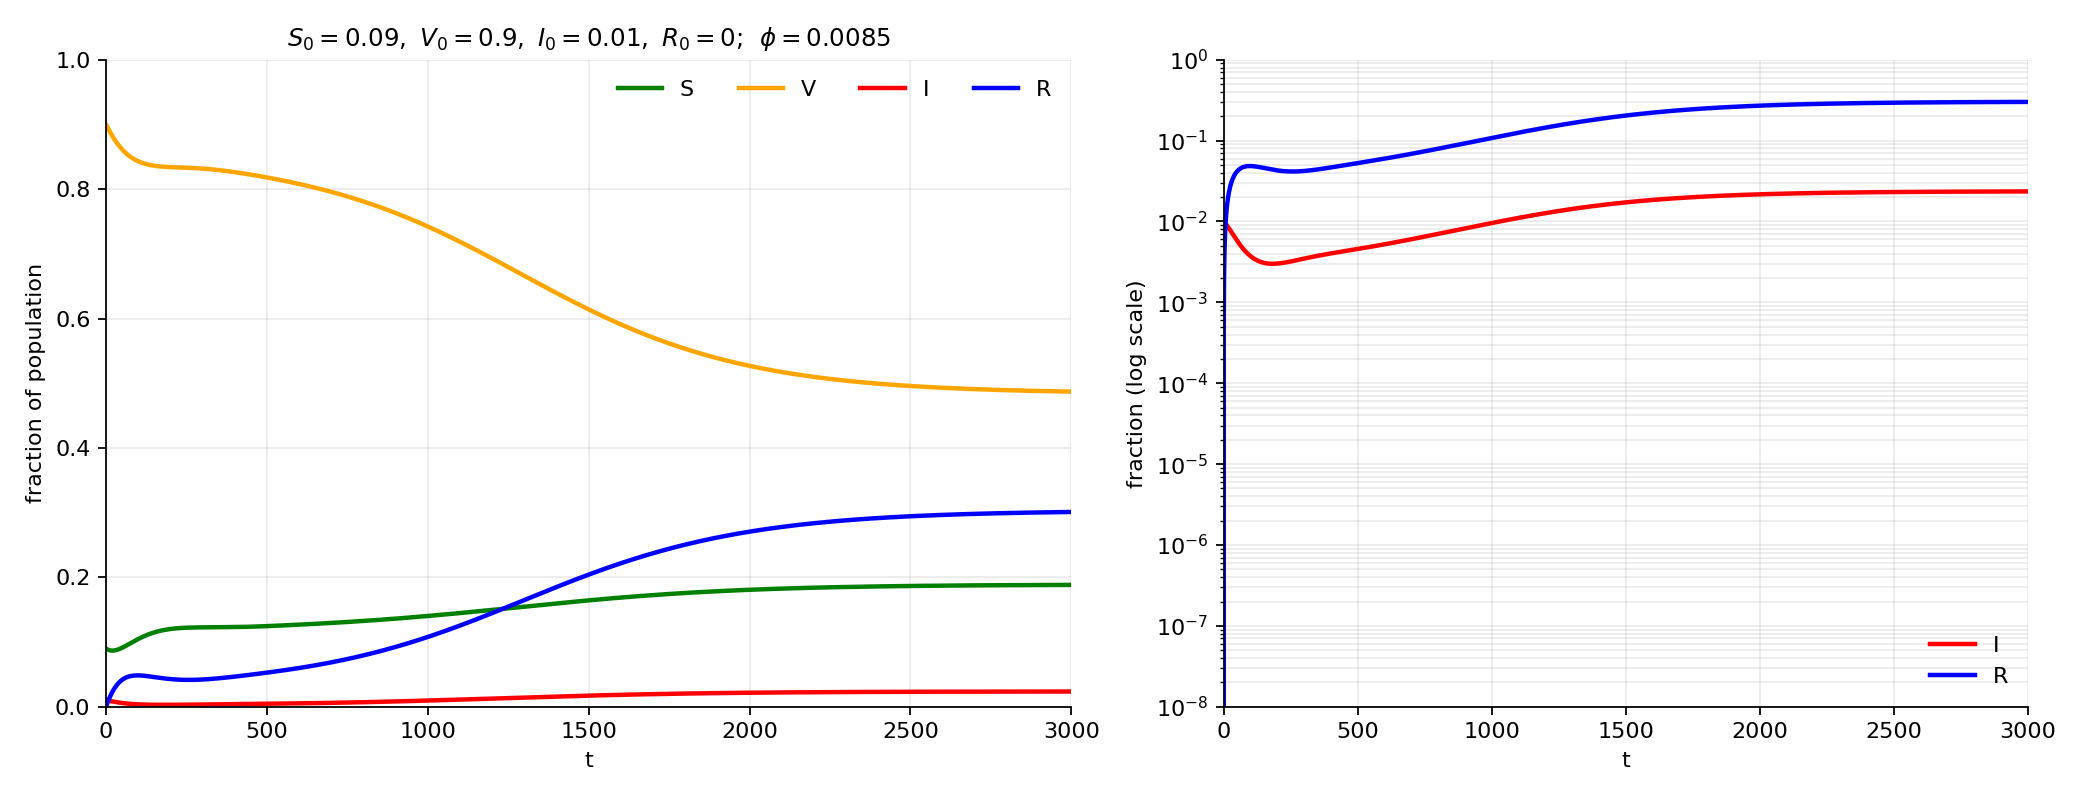
\includegraphics[width=\textwidth]{sim_phi0085_V09.png}
\caption{$\phi=0.0085$, initial condition $S_0=0.09$, $V_0=0.9$, $I_0=0.01$, $R_0=0$. Left: all compartments. Right: $I$ and $R$ on a logarithmic scale.}
\label{fig:V09}
\end{figure}

\emph{Comments.} Although the initial effective reproduction number $\beta(S_0+\sigma V_0)/(\gamma+\mu)\approx0.945$ is below $1$, the run does \emph{not} end at the DFE. The infection first decreases, to a minimum $I\approx0.0030$ near $t\approx182$, and then increases slowly toward the endemic equilibrium: $I=0.02353$ at $t=3000$ and $I=0.023670$ at $t=30000$ (with $V\approx0.484$, $S\approx0.189$, $R\approx0.303$ in the long run). The initial dip is a transient: recovered individuals return to the susceptible class through waning immunity (rate $\psi$), the vaccinated class is depleted through waning vaccine protection (rate $\theta$) and through infection, and the larger susceptible pool allows the infection to grow again. This point therefore lies on the endemic side of the basin boundary computed next.

%=====================================================================
\section{Basin of attraction of the two equilibria}
%=====================================================================

\subsection{Slice and method}

The state space is three-dimensional ($S+V+I+R=1$), so a picture in the $(V_0,I_0)$ plane requires fixing a slice. We use the slice of the previous runs:
\[
R_0=0,\qquad S_0=1-V_0-I_0,\qquad \phi=0.0085 .
\]
For each $V_0\in[0.65,0.99]$ (step $0.0025$) the smallest $I_0$ that leads to the endemic equilibrium was found by bisection on full trajectories (relative tolerance $2\times10^{-4}$). A trajectory was classified as disease-free if $I$ dropped below $10^{-9}$, and as endemic if $I>10^{-4}$ at $t=80000$ (maximum integration time). For $V_0=0.86,\,0.90,\,0.94,\,0.96$ a scan of $200$ values of $I_0$ showed exactly one switch from disease-free to endemic, so the boundary is a single threshold $I_c(V_0)$ in $I_0$ there. A coarse grid scan over $V_0\in[0.65,0.99]$, $I_0\in[0,0.03]$ showed the same pattern.

\subsection{Result}

\begin{figure}[ht]
\centering
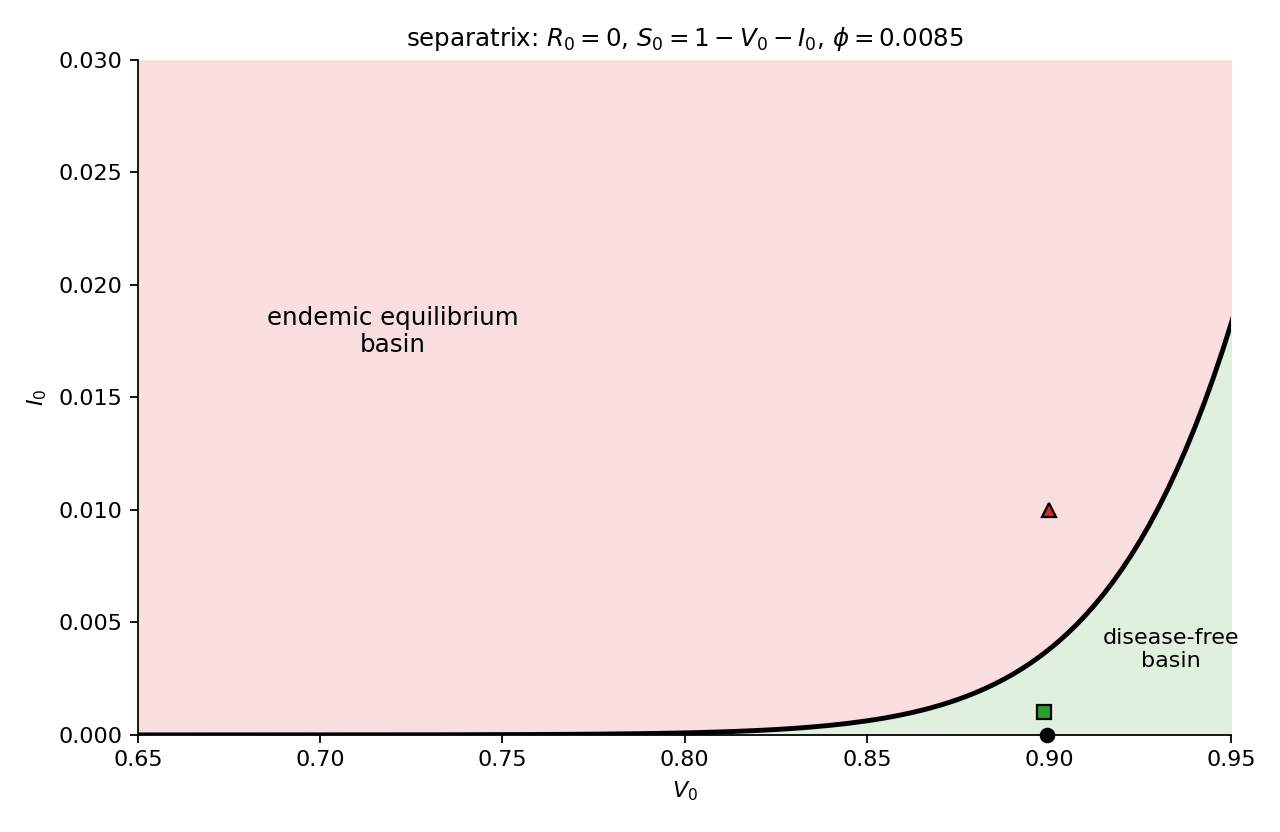
\includegraphics[width=0.85\textwidth]{basin_separatrix_left.png}
\caption{Separatrix between the basins of attraction in the $(V_0,I_0)$ plane, for $R_0=0$, $S_0=1-V_0-I_0$, $\phi=0.0085$. Above the black curve (red) trajectories go to the endemic equilibrium; below it (green) to the disease-free equilibrium. The black dot is the vaccinated DFE ($V^*\approx0.8995$). The green square $(0.8986,0.001)$ and the red triangle $(0.9,0.01)$ are initial conditions from Sections~3 and~4 that went to the DFE and to the endemic state, respectively.}
\label{fig:basin}
\end{figure}

Selected values of the threshold are
\begin{center}
\begin{tabular}{cc}
\toprule
$V_0$ & $I_c(V_0)$\\
\midrule
$0.65$ & $2.0\times10^{-7}$\\
$0.80$ & $9.0\times10^{-5}$\\
$0.90$ & $3.8\times10^{-3}$\\
$0.95$ & $1.83\times10^{-2}$\\
\bottomrule
\end{tabular}
\end{center}

\emph{Comments.}
\begin{itemize}
\item The threshold increases steeply with $V_0$; on a logarithmic scale it is nearly a straight line, so $I_c$ grows roughly exponentially with $V_0$. It is strictly positive for all $V_0$ shown (about $2\times10^{-7}$ at $V_0=0.65$), so on the linear scale of Figure~\ref{fig:basin} it hugs the horizontal axis for $V_0\lesssim0.85$.
\item The more vaccinated the initial population, the larger the infection needed to reach the endemic state. Outside the range plotted, the curve reaches $I_0=0.03$ at $V_0\approx0.968$.
\item The earlier test points are consistent with the curve: $I_c(0.9)\approx0.0038$, so $I_0=0.001$ falls in the disease-free basin and $I_0=0.01$ in the endemic one.
\item The curve depends on the slice $R_0=0$ and on the value of $\phi$; other choices would shift it.
\end{itemize}

%=====================================================================
\section{Summary}
%=====================================================================

\begin{enumerate}
\item With $\phi=0.0085$ ($r\approx0.9813\in(r_2,1)$) the model has two stable equilibria: the vaccinated disease-free state ($S^*\approx0.1005$, $V^*\approx0.8995$) and an endemic state ($S\approx0.189$, $V\approx0.484$, $I\approx0.0237$, $R\approx0.303$). The endemic value of $I$ agrees with the root $I_1(r)$ of the equilibrium quadratic.
\item Initial conditions with $V_0=0$ always converged to the endemic state in the experiments, even for very small $I_0$.
\item Starting at the vaccinated DFE with $I_0=0.001$ the infection dies out; with $I_0=0.01$ it reaches the endemic state.
\item From $V_0=0.9$, $I_0=0.01$ the infection first declines and then rebounds to the endemic state.
\item The basin separatrix in the $(V_0,I_0)$ plane (slice $R_0=0$) is a single increasing curve $I_c(V_0)$, from about $2\times10^{-7}$ at $V_0=0.65$ to $1.83\times10^{-2}$ at $V_0=0.95$.
\end{enumerate}

\end{document}
